\section{Einleitung}

Das Projekt basiert auf dem FlexSort, eine optischen Bandsortieranlage für Schüttgut am Fraunhofer IOSB. Die Sortieranlage kann Schüttgut mit Hilfe einer Flächenkamera optisch klassifizieren und mittels Druckluftdüsen voneinander trennen. Damit eine konstante und gleichverteilte Menge von Schüttgut auf dem Band liegt, wird über ein Rüttler das Material freigegeben und rutscht über eine Rutsche auf das Band. Die nachfolgenden Abbildungen zeigen den Aufbau des FlexSorts,

%\begin{figure}[htb]
%	\centering
%	\begin{minipage}[t]{0.49\linewidth}
%		\centering
%		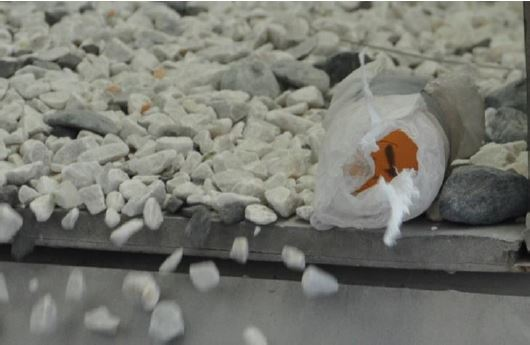
\includegraphics[width=1\linewidth]{images/k4-polsterfolie.JPG}
%		\caption{Variante 1: Kapsel in Polsterfolie eingepackt}
%		\label{fig:k4_polsterfolie}
%	\end{minipage}% <- sonst wird hier ein Leerzeichen eingefügt
%	\hfill
%	\begin{minipage}[t]{0.49\linewidth}
%		\centering
%		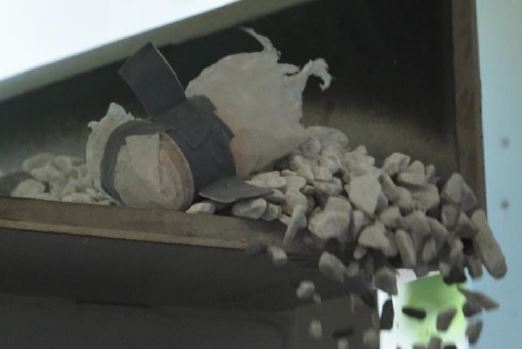
\includegraphics[width=\linewidth]{images/k4-fluegel.JPG}
%		\caption{Beispielbild mit einer sehr langen Beschriftung, die nicht in eine Zeile hinein passt}
%		\label{fig:k4_fluegel}
%	\end{minipage}
%\end{figure}
%
%\begin{figure}[htb]
%	\centering
%	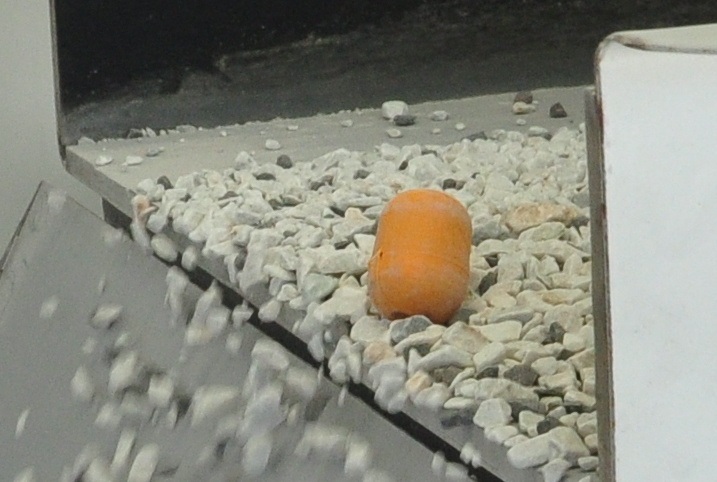
\includegraphics[width=0.49\linewidth]{images/k4-kapsel.JPG}
%	\caption{Beispielbild}
%	\label{fig:k4_kapsel}
%\end{figure}

%TODO eigenes Bild, ansonsten korrekte Quellenangabe mit URL + Footnote

Da die Klassifizierung und das Ausblasen von Teilchen etwas verzögert stattfinden, ist eine zeitlich gut geplante Aktivierung der Druckluftdüsen notwendig, um die Anlage möglichst kostensparend und effizient zu betreiben. Hierfür muss die genaue Position der auszusortierenden Teilchen zum Zeitpunkt der Düsenüberquerung ermittelt werden. Dabei ist zu beachten, dass sich das Schüttgut vom Klassifizierungszeitpunkt bis zum Zeitpunkt des Ausblasens auf dem Band bewegt. Die Bewegung der Teilchen kann unter Umständen von einzelnen Parametern der Anlage beeinflusst werden und wirkt sich dadurch auf das Sortierergebnis aus. Beispielsweise kann die Geschwindigkeit des Bandes dazu führen, dass die Teilchen darauf springen oder der Rüttler durch ungünstige Vibrationsbewegungen keine konstante Menge von Teilchen über die Rutsche auf das Band frei gibt. 

In diesem Projekt soll eine Möglichkeit gefunden werden, den Prozess des Sortierens von Schüttgut genauer zu verstehen und dadurch weitere Optimierungen an der Anlage und im Prozess vornehmen zu können. So könnte ein stabileres Sortierergebnis erreicht werden. Neben den rein optisch gewonnen Daten können weitere Messwerte durch andere Verfahren unterstützend sein. In diesem Projekt soll dies mit Hilfe eines instrumentierten Schüttguts passieren, über den Bewegungsdaten gesammelt und ausgewertet werden können. Es soll untersucht werden, ob sich in den gewonnen Daten bestimmte Bewegungsmuster erkennen lassen, die auf einzelne Anlagenmodule zurückgeführt werden können. Gegebenenfalls lassen sich zwischen den Anlagenmodulen verschiedene Korrelationen erkennen, die zukünftig zur Optimierung der Anlage genutzt werden können. Darüber hinaus könnte ein Qualitätsmaß erstellt werden, anhand dessen die gewählten Parameter der Anlage bewertet werden.

